\section{The \specdx Approach}
\label{sec:approach}

\Cref{fig:pipeline} gives an overview. \specdx works in rounds, and each round has five steps:
\begin{enumerate}[leftmargin=*]
\item It picks a scenario (\cref{sec:approach-scenarios}).
\item It runs a pilot of the population on that scenario, and the full population only if the pilot looks informative.
\item It reads each run at the level of items and cells (\cref{sec:approach-observe}).
\item It fits two statistical models: an act model that says where the evidence is reliable (\cref{sec:approach-act}), and the anchored cell model that says what $\Tell$ admits at each cell (\cref{sec:approach-model}).
\item It turns the posteriors into typed findings, which it backs with logical witnesses and localises in $\Tell$ (\cref{sec:approach-typing,sec:approach-localise}).
\end{enumerate}
The loop is \emph{anytime}: stopping it at any point yields a report.

\begin{figure}[t]
\centering
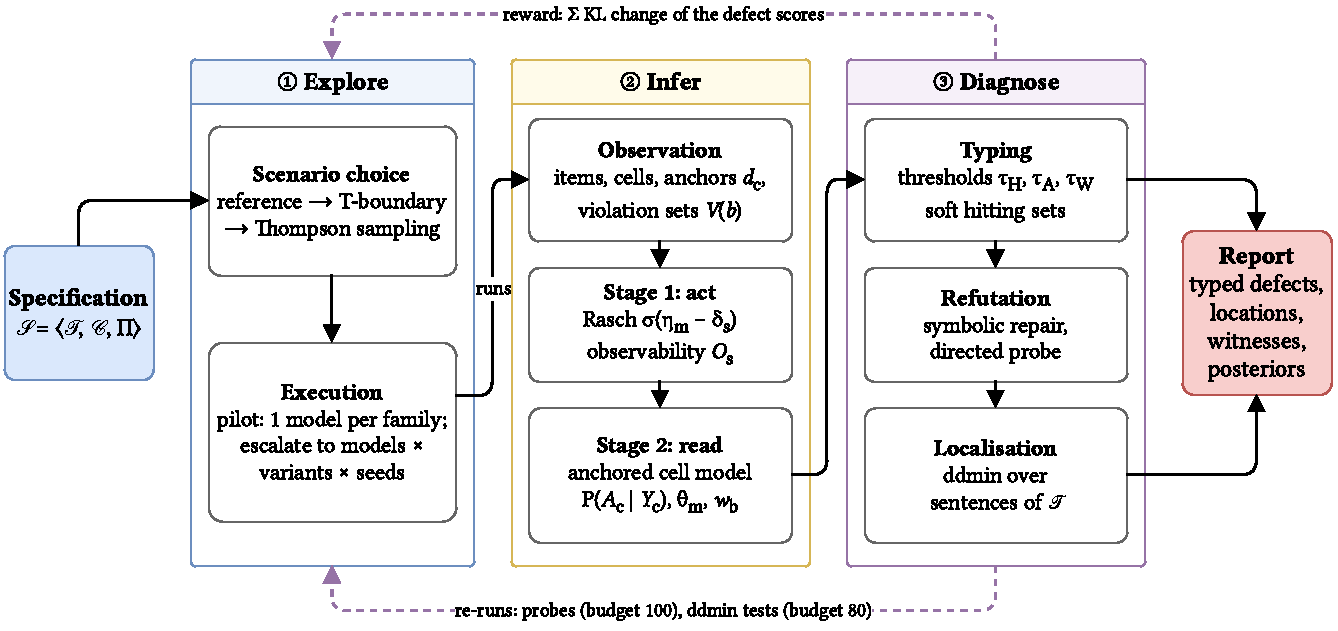
\includegraphics[width=\textwidth]{figures/drawio/pipeline.pdf}
\caption{Overview of \specdx. Each round explores a scenario, infers what the population's runs say about every cell, and diagnoses typed defects. Solid arrows show one round. Dashed arrows show the feedback: the change in the defect scores rewards the scenario choice, and refutation and localisation request further runs within their own budgets.}
\label{fig:pipeline}
\end{figure}

\subsection{Execution and observation}
\label{sec:approach-observe}

\paragraph{Neutral harness.} Each interpreter runs the process step by step with the tools of the step's digital employee. It works against a real PostgreSQL database with the specification's guardrails installed. It reads $\Tell$ through a retrieval tool: BM25 over 300-word chunks, $k=5$ per query.

Small open models sometimes write a tool call as text, or end a step without acting. A neutral harness handles both cases, and its texts contain no business value or rule:
\begin{itemize}[leftmargin=*]
\item \textbf{Tool calls written as text.} A call written as text is parsed and executed only if it names one of the step's tools and its arguments validate against that tool's schema.
\item \textbf{Steps that end without acting.} The harness may remind the model at most twice that it has not used a tool. The model remains free to answer that it is done.
\end{itemize}

\paragraph{What is recorded.} For each run, \specdx records the behaviour $b$, its violation set $V(b)$ from~\eqref{eq:violset}, and, for each item $s$, the act indicator
\begin{equation}
\label{eq:act}
a_{bs}=\one\bigl[\text{step } s \text{ ended } \textsf{done}\bigr]\cdot\one\bigl[\text{$b$ wrote at least one new row or event in the slice of } s\bigr].
\end{equation}
A step that errs, times out, is refused or writes nothing has $a_{bs}=0$.

For every cell $c$ that item $s$ may write, an acted behaviour also contributes a reading $y_{bc}$. Readings are normalised syntactically only, by Unicode NFC, trimming, whitespace folding, casefolding and canonical numerals. No semantic mapping is applied, so \textit{draft} and \textit{Nháp} remain different readings, and the model decides whether one of them is an interpreter error.

Rows are matched to golden rows by natural key. A key column whose golden values never occur in $\Tell$ is treated as generated by the executor, and its rows are matched on the remaining locked foreign keys instead.

\subsection{Stage 1: who acts, and where}
\label{sec:approach-act}

A model that never acts at an item says nothing about how it reads the item. Treating silence as disagreement was the main failure of our first prototype. \specdx therefore separates \emph{acting} from \emph{reading}. Stage 1 is a Rasch model~\cite{rodriguez2021evaluation,lalor2016building} of the act indicator:
\begin{equation}
\label{eq:rasch}
\Prob(a_{bs}=1)=\sigma\bigl(\eta_{m(b)}-\delta_s\bigr),
\end{equation}
where $\eta_m$ is model $m$'s capability to act and $\delta_s$ is the difficulty of item $s$. It is fitted by penalised maximum likelihood with an $L_2$ penalty $\lambda=1$ on $\eta$ and $\delta$, and with $\sum_s\delta_s=0$ fixed. The \emph{observability} of an item is the population's mean probability of acting,
\begin{equation}
\label{eq:observability}
O_s=\frac{1}{|\Models|}\sum_{m\in\Models}\sigma(\eta_m-\delta_s).
\end{equation}
An item is \emph{observable} when $O_s\ge\omega=0.3$ and at least $m_{\min}=3$ behaviours acted on it. Only acted behaviours contribute readings, and a finding whose clauses are not all relevant to observable items goes to an \emph{Unobservable} list. This list is reported, but it is never typed or scored. \Cref{prop:noaction} in \cref{sec:theory} shows that abstaining is the only calibrated answer in that case.

\subsection{Stage 2: the anchored cell model}
\label{sec:approach-model}

The anchored cell model is the core of \specdx. It answers \textbf{Q1}: given the readings of a cell by interpreters of differing competence, which readings does $\Tell$ admit?

\paragraph{Candidate values and latent sets.} For each cell $c$, the candidate set $V_c$ is built in three steps:
\begin{enumerate}[leftmargin=*]
\item it starts with the anchor $d_c$, if the cell is anchored;
\item it adds the most frequent observed readings, up to $K_{\max}=6$ values in all;
\item it adds one bucket \other for every remaining reading.
\end{enumerate}
The latent set $A_c$ ranges over
\begin{equation}
\label{eq:sets}
\Sets_c=\bigl\{\{x\}:x\in V_c^\circ\bigr\}\;\cup\;\bigl\{\{x,y\}:x\neq y\in V_c^\circ\bigr\}\;\cup\;\{\emptyset\},\qquad V_c^\circ=V_c\setminus\{\other\},
\end{equation}
which gives at most $6+15+1=22$ candidate sets per cell. \other never belongs to $A_c$.

\paragraph{Prior over sets.} We call the three ways a set can depart from the anchor its \emph{defect forms}:
\begin{itemize}[leftmargin=*]
\item \emph{mis}, a single value other than $d_c$;
\item \emph{amb}, a two-value set;
\item $\emptyset$, the empty set.
\end{itemize}
On an anchored cell, the prior keeps mass $1-\pi$ on the anchor and splits $\pi$ among the forms:
\begin{equation}
\label{eq:setprior}
\Prob(A_c=A)=
\begin{cases}
1-\pi, & A=\{d_c\},\\[2pt]
\pi\,s_f\,/\,N_f(c), & A \text{ of form } f\in\{\textit{mis},\textit{amb},\emptyset\},
\end{cases}
\end{equation}
where $s_{\textit{mis}}+s_{\textit{amb}}+s_\emptyset=1$ and $N_f(c)$ is the number of candidate sets of form $f$ at $c$. On an unanchored cell, the single values share $1-\pi$ uniformly, and $\pi$ is split between pairs and $\emptyset$ in the ratio $s_{\textit{amb}}:s_\emptyset$.

\paragraph{Reading model.} Let behaviour $b$ come from model $m=m(b)$. Its \emph{accuracy} at cell $c$ is
\begin{equation}
\label{eq:accuracy}
p_{m,c}=\sigma\bigl(\alpha_m-\beta_{g(c)}\bigr),
\end{equation}
where $\alpha_m$ is the model's ability and $\beta_g$ is the difficulty of the cell's group. The group $g(c)$ is the column of a value cell (pooled over rows and scenarios), the kind and reference of an event cell, and the clause of a constraint cell. Given $A_c$, the reading $y_{bc}$ is generated by
\begin{equation}
\label{eq:reading}
\Prob\bigl(y_{bc}=y\mid A_c=A\bigr)=
\begin{cases}
p_{m,c}\,\dfrac{\one[y\in A]}{|A|}+\bigl(1-p_{m,c}\bigr)\,\tilde\varepsilon_c^{A}(y), & A\neq\emptyset,\\[8pt]
\varepsilon_c(y), & A=\emptyset,
\end{cases}
\qquad
\tilde\varepsilon_c^{A}(y)=\frac{\varepsilon_c(y)\,\one[y\notin A]}{1-\varepsilon_c(A)} .
\end{equation}
In words: with probability $p_{m,c}$, the interpreter reads the cell faithfully and picks one of the admissible values uniformly. Otherwise it errs, and its error is drawn from a cell-specific error distribution $\varepsilon_c$ \emph{restricted to values outside $A$}. When $\Tell$ says nothing ($A=\emptyset$), no reading is faithful, and all models draw from the same $\varepsilon_c$.

Three design choices distinguish~\eqref{eq:reading} from the classical Dawid--Skene~\cite{dawid1979maximum} and GLAD~\cite{whitehill2009whose} models.
\begin{enumerate}[leftmargin=*,label=(\roman*)]
\item \textbf{Set-valued truth.} The truth is a set, which may hold two values or none. This is what lets the model express ambiguity and silence.
\item \textbf{Accuracy is a probability of landing in the truth.} Because the error distribution is truncated to $V_c\setminus A$, error mass can never sit on an admissible value, and $p_{m,c}$ is exactly $\Prob_m(y\in A)$. In an earlier version, the error distribution was allowed to cover the admissible values. The data then fitted a whole one-parameter family of (accuracy, error) pairs equally well, and accuracy collapsed to the share of the plurality class. The truncation removes that degeneracy.
\item \textbf{The specification is one more rater.} The anchor enters only through the prior~\eqref{eq:setprior}, so a cell whose anchor is consistently contradicted by competent readers can move its posterior away from $d_c$.
\end{enumerate}

\paragraph{Parameter priors.} The parameters receive weakly informative priors:
\begin{equation}
\label{eq:paramprior}
\alpha_m\sim\Norm(\mu_\alpha,\sigma_\alpha^2),\qquad
\beta_g\sim\Norm(0,\tau^2),\qquad
\varepsilon_c\sim\Dir\bigl(\kappa\,u_c\bigr),
\end{equation}
where $u_c$ is the flat distribution over $V_c$ and $\kappa=10$. The flat pool has a specific job. A free per-cell $\varepsilon_c$ lets the silence hypothesis $A_c=\emptyset$ fit any sharp split or mode, and in our simulation spikes it absorbed almost every true ambiguity. Pulling $\varepsilon_c$ towards a flat profile makes silence predict flat readings, so a sharp split identifies a pair and a sharp mode identifies a value (\cref{thm:t2prime}). The pool is a regularisation, not a claim that errors are flat: real errors concentrate, and \cref{sec:theory} and the simulation study examine what happens then.

\Cref{fig:graphical} summarises the generative model as a plate diagram.

\begin{figure}[t]
\centering
\resizebox{\textwidth}{!}{% Plate diagram of the anchored cell model.
\begin{tikzpicture}[
  every node/.style={font=\footnotesize},
  latent/.style={circle, draw, minimum size=8.5mm, inner sep=0pt},
  obs/.style={latent, fill=gray!25},
  param/.style={rectangle, inner sep=1pt},
  arr/.style={-{Latex[length=1.8mm]}, thick},
  plate/.style={draw, rounded corners=3pt, inner sep=6pt}]
\node[obs] (y) at (0,0) {$y_{bc}$};
\node[latent] (A) at (0,1.7) {$A_c$};
\node[obs] (d) at (-1.6,2.9) {$d_c$};
\node[param] (pi) at (1.6,2.9) {$\pi,\ s_f$};
\node[latent] (eps) at (2.0,0.9) {$\varepsilon_c$};
\node[param] (kap) at (3.6,0.9) {$\kappa,\ u_c$};
\node[latent] (al) at (-3.4,0) {$\alpha_m$};
\node[param] (mua) at (-5.2,0) {$\mu_\alpha,\sigma_\alpha$};
\node[latent] (be) at (-1.9,-1.75) {$\beta_g$};
\node[param] (tau) at (-3.7,-1.75) {$\tau$};
\node[latent, dashed] (p) at (-1.6,0.55) {$p_{m,c}$};
\draw[arr] (d) -- (A); \draw[arr] (pi) -- (A);
\draw[arr] (A) -- (y); \draw[arr] (eps) -- (y); \draw[arr] (kap) -- (eps);
\draw[arr] (mua) -- (al); \draw[arr] (tau) -- (be);
\draw[arr] (al) -- (p); \draw[arr] (be) -- (p); \draw[arr] (p) -- (y);
\node[plate, fit=(y), label={[font=\scriptsize]below right:acted $b$}] (pb) {};
\node[plate, fit=(pb)(A)(d)(eps)(p), label={[font=\scriptsize]above right:cells $c\in\Cells$}] {};
\node[plate, fit=(al), label={[font=\scriptsize]below:models $m\in\Models$}] {};
\node[plate, fit=(be), label={[font=\scriptsize]below:groups $g$}] {};
\node[align=left, font=\scriptsize, anchor=west] at (4.6,1.9) {%
  $A_c\in\Sets_c$: admissible readings\\
  $p_{m,c}=\sigma(\alpha_m-\beta_{g(c)})$ (deterministic)\\
  $y\mid A\neq\emptyset$: faithful w.p.\ $p_{m,c}$,\\
  \quad otherwise $\varepsilon_c$ restricted to $V_c\setminus A$\\
  $y\mid A=\emptyset$: drawn from $\varepsilon_c$};
\end{tikzpicture}
}
\caption{Plate diagram of the anchored cell model. Shaded nodes are observed: the readings $y_{bc}$ and the anchors $d_c$. The anchor enters only through the prior on the latent set $A_c$. Accuracy $p_{m,c}$ is a deterministic function of model ability and group difficulty.}
\label{fig:graphical}
\end{figure}

\paragraph{Posterior.} Let $\Theta=(\alpha,\beta,\varepsilon)$ and let $Y_c=\{y_{bc}\}$ be the readings of cell $c$ by acted behaviours. Under conditional independence of readings given $A_c$ and $\Theta$, the cell-level posterior is
\begin{equation}
\label{eq:post}
\Prob(A_c=A\mid Y_c,\Theta)=\frac{\Prob(A_c=A)\prod_{b}\Prob(y_{bc}\mid A,\Theta)}{\sum_{A'\in\Sets_c}\Prob(A_c=A')\prod_{b}\Prob(y_{bc}\mid A',\Theta)},
\end{equation}
and \specdx maximises the log posterior with every $A_c$ summed out,
\begin{equation}
\label{eq:map}
\mathcal{L}(\Theta)=\sum_{c\in\Cells}\log\sum_{A\in\Sets_c}\Prob(A_c=A)\prod_{b}\Prob(y_{bc}\mid A,\Theta)\;+\;\log p(\alpha)+\log p(\beta)+\log p(\varepsilon).
\end{equation}

\paragraph{Fitting by EM.} \specdx finds a MAP estimate of $\Theta$ by expectation--maximisation~\cite{dempster1977maximum}.

\emph{E-step.} For each cell, compute the posterior~\eqref{eq:post} over all candidate sets. Then compute, for each reading, the probability that it is faithful,
\begin{equation}
\label{eq:faithful}
r_{bc}=\sum_{A\neq\emptyset}\Prob(A_c=A\mid Y_c,\Theta)\cdot\frac{p_{m,c}\,\one[y_{bc}\in A]/|A|}{p_{m,c}\,\one[y_{bc}\in A]/|A|+(1-p_{m,c})\,\tilde\varepsilon_c^A(y_{bc})},
\end{equation}
and the probability that the cell is not silent, $q_c=1-\Prob(A_c=\emptyset\mid Y_c,\Theta)$.

\emph{M-step for ability and difficulty.} The expected complete-data log posterior in $(\alpha,\beta)$ is a penalised logistic regression. In it, each reading is a trial of accuracy with weight $q_c$ and fractional success $r_{bc}$:
\begin{equation}
\label{eq:mstep-ab}
(\alpha,\beta)\leftarrow\argmax_{\alpha,\beta}\sum_{c}\sum_{b}\Bigl[r_{bc}\,\eta_{m(b),c}-q_c\log\bigl(1+e^{\eta_{m(b),c}}\bigr)\Bigr]-\frac{\|\alpha-\mu_\alpha\|^2}{2\sigma_\alpha^2}-\frac{\|\beta\|^2}{2\tau^2},
\qquad \eta_{m,c}=\alpha_m-\beta_{g(c)} .
\end{equation}
\specdx solves~\eqref{eq:mstep-ab} by damped Newton steps, using the Schur complement of the diagonal $\beta$ block.

\emph{M-step for the error distributions.} An error reading under $A\neq\emptyset$ is a draw from $\varepsilon_c$ after any draws that fell inside $A$ have been rejected. The exact EM step therefore adds the expected rejected draws to the observed error counts. Let $N_c^{\textit{err}}(A)$ be the number of readings of $c$ outside $A$. The expected rejected draws on a value $k$ are
\begin{equation}
\label{eq:mstep-eps-rej}
R_c(k)=\sum_{A\ni k}\Prob(A_c=A\mid Y_c,\Theta)\,N_c^{\textit{err}}(A)\,\frac{\varepsilon_c(k)}{1-\varepsilon_c(A)} .
\end{equation}
The update is then
\begin{equation}
\label{eq:mstep-eps}
\varepsilon_c(k)\leftarrow\frac{E_c(k)+R_c(k)+\kappa\,u_c(k)}{\sum_{k'}\bigl[E_c(k')+R_c(k')\bigr]+\kappa},
\qquad E_c(k)=\sum_b(1-r_{bc})\,\one[y_{bc}=k] .
\end{equation}
This is the posterior mean under $\Dir(\kappa u_c)$, so the prior acts as exactly $\kappa$ pseudo-counts towards the flat pool.

\emph{Initialisation and stopping.} The likelihood~\eqref{eq:map} is multimodal. On our base data, more than half of the anchored cells are read off their anchor by every model, because nobody writes those rows. That is beyond the breakdown point of the median estimator in \cref{thm:t3}. EM therefore runs from five starts and keeps the fit with the highest $\mathcal{L}$:
\begin{itemize}[leftmargin=*]
\item the median start of \cref{thm:t3};
\item a common ability $\alpha_m\in\{0,1,2,3\}$ for every model.
\end{itemize}
Every start sets $\beta_g=0$ and $\varepsilon_c=u_c$. EM stops when the largest parameter change falls below $10^{-6}$, or after 200 iterations. Non-convergence is reported, never hidden.

\paragraph{Outputs.} The fit yields three kinds of output:
\begin{itemize}[leftmargin=*]
\item \textbf{Per cell:} the posterior over $A_c$, its MAP set and the posterior mass of each defect form.
\item \textbf{Per model:} the ability $\alpha_m$ and the accuracy $\theta_m=\sigma(\alpha_m)$ at a cell of median difficulty.
\item \textbf{Per behaviour:} a weight
\begin{equation}
\label{eq:weight}
w_b=\frac{1}{|\Cells_b|}\sum_{c\in\Cells_b}r_{bc},
\end{equation}
the mean probability that $b$'s readings are faithful, taken over the cells $\Cells_b$ it read.
\end{itemize}
No component of \specdx is switched on or off by a hard threshold on competence. Posterior quantities are used as weights throughout.

\subsection{Typing}
\label{sec:approach-typing}

This subsection answers \textbf{Q2}: how the posteriors become typed findings with witnesses. \Cref{fig:typing} summarises the decision flow; the paragraphs below give the details.

\begin{figure}[t]
\centering
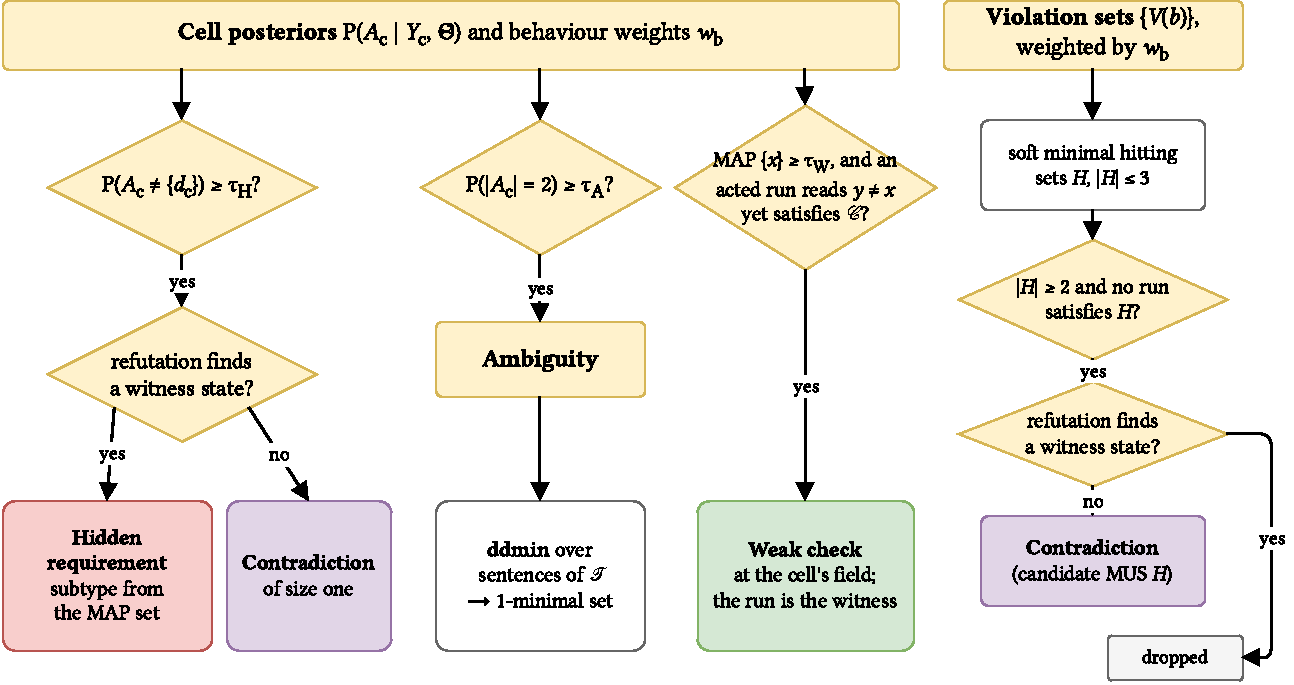
\includegraphics[width=\textwidth]{figures/drawio/typing.pdf}
\caption{Typing. The cell posteriors give hidden requirements, contradictions of size one, ambiguities and weak checks; the weighted violation sets give contradictions of two or more clauses. Every contradiction requires a failed refutation, and every ambiguity is localised in $\Tell$ by ddmin.}
\label{fig:typing}
\end{figure}

\paragraph{Hidden requirements and contradictions of size one.} An anchored cell is a candidate when its anchor is unlikely to be the whole truth:
\begin{equation}
\label{eq:hid-cand}
\Prob\bigl(A_c\neq\{d_c\}\mid Y_c,\hat\Theta\bigr)\ge\tau_H .
\end{equation}
The candidate then goes to \emph{refutation} (described below), which searches for a state that satisfies every applicable clause except the cell's own clause, together with a value of the cell other than $d_c$.
\begin{itemize}[leftmargin=*]
\item \textbf{A state is found.} The finding is a hidden requirement at the cell's clause, and its subtype follows the MAP form: mis-key for $\{a\}$, ambiguous-pick for a pair, unstated for $\emptyset$.
\item \textbf{No state is found.} The clause is a contradiction of size one.
\end{itemize}

\paragraph{Contradictions of two or more clauses.} If $b\models\Chk(\pi)\setminus V(b)$, then $V(b)$ is a \emph{correction set}: removing it makes the remaining clauses satisfiable. By the minimal hitting set duality of Reiter~\cite{reiter1987theory} and Liffiton and Sakallah~\cite{liffiton2008algorithms}, every minimal unsatisfiable subset is a minimal hitting set of the minimal correction sets. \specdx therefore treats every run as a free sample of a correction set, weighted by $w_b$. Let $\mathcal{V}_\pi=\{V(b)\}$ be the violation sets of the acted behaviours on $\pi$; each $V(b)$ is restricted to clauses relevant to items where $b$ acted. A set $H\subseteq\Chk(\pi)$ is a \emph{soft hitting set} when
\begin{equation}
\label{eq:sofths}
\frac{\sum_{b}w_b\,\one\bigl[H\cap V(b)\neq\emptyset\bigr]}{\sum_b w_b\,\one\bigl[V(b)\neq\emptyset\bigr]}\ge 1-\tau_{\textit{hs}},\qquad |H|\le 3 .
\end{equation}
\specdx enumerates minimal soft hitting sets with PySAT's \textsc{Hitman}~\cite{ignatiev2018pysat}, with $\tau_{\textit{hs}}=0.05$. It drops behaviours whose weight share is below $0.01$. A set $H$ with $|H|\ge 2$ becomes a contradiction candidate when every clause of $H$ is satisfied individually by some behaviour but no behaviour satisfies all of them together. The candidate is reported only if refutation fails. \Cref{fig:hitting} works through a small example.

\begin{figure}[t]
\centering
\resizebox{\textwidth}{!}{% Runs as sampled correction sets; a minimal hitting set is a candidate MUS.
\begin{tikzpicture}[
  every node/.style={font=\footnotesize},
  c/.style={minimum width=0.75cm, minimum height=0.48cm, draw=gray!50},
  hl/.style={c, fill=purple!15},
  arr/.style={-{Latex[length=2mm]}, thick},
  box/.style={draw, rounded corners=2pt, align=center, inner sep=4pt}]
\foreach \j/\n in {1/1,2/2,3/3,4/4} \node at (\j*0.75,0.5) {$\varphi_{\n}$};
\node at (4.15,0.5) {$w_b$};
\foreach \r/\row/\w in {1/{0,1,0,0}/0.9, 2/{0,0,1,0}/0.8, 3/{0,1,0,1}/0.7, 4/{1,0,1,0}/0.6, 5/{1,1,0,0}/0.9} {
  \node[anchor=east] at (0.3,-0.48*\r+0.48) {$V(b_{\r})$};
  \foreach \v [count=\j] in \row {
    \ifnum\j=2 \def\sty{hl}\else\ifnum\j=3 \def\sty{hl}\else\def\sty{c}\fi\fi
    \node[\sty] at (\j*0.75,-0.48*\r+0.48) {\ifnum\v=1 $\bullet$\fi};
  }
  \node at (4.15,-0.48*\r+0.48) {\w};
}
\node[font=\scriptsize, align=center, text width=4.2cm] at (2.0,-2.45) {each run $b$ satisfies $\Chk\setminus V(b)$, so $V(b)$ is a correction set};
\node[box, fill=purple!15] (H) at (7.0,-0.5) {minimal hitting set\\$H=\{\varphi_2,\varphi_3\}$\\covers all weight};
\node[box] (R) at (10.0,-0.5) {refutation: search\\for $w\models\{\varphi_2,\varphi_3\}$};
\node[box, fill=purple!25] (C) at (10.0,-2.0) {no witness:\\\Dcon $\{\varphi_2,\varphi_3\}$};
\node[box, fill=gray!10] (D) at (7.0,-2.0) {witness found:\\candidate dropped};
\draw[arr] (4.6,-0.5) -- (H);
\draw[arr] (H) -- (R);
\draw[arr] (R) -- (C);
\draw[arr] (R.south west) -- (D.north east);
\end{tikzpicture}
}
\caption{Runs as sampled correction sets. Every run violates $\varphi_2$ or $\varphi_3$, and each of the two is satisfied by some run, so $H=\{\varphi_2,\varphi_3\}$ is a minimal hitting set and a candidate MUS. It is reported as a contradiction only if refutation finds no state that satisfies both clauses.}
\label{fig:hitting}
\end{figure}

\paragraph{Refutation.} Refutation searches for a witness state $w$ with $w\models M$, along two routes.
\begin{itemize}[leftmargin=*]
\item \textbf{Symbolic repair.} Starting from the behaviours that violate the fewest clauses of $M$, a local search over the locked fields proposes edits. Each proposal is materialised in PostgreSQL inside a savepoint, so that derived values such as \texttt{fn\_reconcile} are computed by the real system. The search stops after at most 200 clause evaluations.
\item \textbf{Directed probe.} $\Tell$ is augmented with the goal of reaching a state that satisfies $M$, written from the clause descriptions. The three interpreters with the highest weight each make three attempts.
\end{itemize}
Refutation is sound: a returned witness proves that $M$ is satisfiable (\cref{prop:refute}). The reverse direction holds only probabilistically, so every contradiction is reported with the number of failed attempts.

\paragraph{Ambiguity.} A cell is reported as an ambiguity when
\begin{equation}
\label{eq:amb}
\Prob\bigl(|A_c|=2\mid Y_c,\hat\Theta\bigr)\ge\tau_A .
\end{equation}
Following \cref{def:defects}, an ambiguity whose pair excludes or includes the anchor is reported together with the corresponding hidden requirement.

\paragraph{Weak checks.} A cell $c$ is a weak-check candidate when two conditions hold:
\begin{enumerate}[leftmargin=*,label=(\roman*)]
\item its MAP set is a single value $\{x\}$ with posterior at least $\tau_W$;
\item some acted behaviour $b$ reads $y_{bc}\neq x$, yet satisfies every clause of $\Chk$ relevant to the item. This is checked symbolically on $b$'s state.
\end{enumerate}
Then $b$ witnesses~\eqref{eq:def-weak}: the population says $b$ is not admissible at $c$, and still no clause objects. The finding is located at the cell's column, or at the event's (kind, ref). Unanchored cells are the main source of weak checks. A weak check is suppressed on a cell that already reports a hidden requirement.

\paragraph{Differential reporting.} When a specification is compared with a reference version, as in the mutation study, only findings that are absent from the reference's report are kept. This applies the matching rules of \cref{sec:eval-design}.

\subsection{Localising ambiguity in the text}
\label{sec:approach-localise}

An ambiguity is only actionable if the author knows which sentences cause it. \specdx localises each reported ambiguity by delta debugging (ddmin)~\cite{zeller2002simplifying} over the sentences of $\Tell$ retrieved for the item's step. Let $T_s$ be those sentences. A test on a subset $U\subseteq T_s$ removes $U$ from $\Tell$ and re-runs one behaviour per (acting model, Tell variant) at seed 1. The oracle keeps the fitted $\hat\Theta$ fixed and asks whether the split persists:
\begin{equation}
\label{eq:ddmin-oracle}
\textsc{Test}(U)=\one\Bigl[\Prob\bigl(|A_c|=2\mid Y_c^{\Tell\setminus U},\hat\Theta\bigr)\ge\tau_A\Bigr].
\end{equation}
ddmin returns a 1-minimal set of sentences whose \emph{presence} is needed for the split. Its cost is $O(\log|T_s|)$ tests in favourable cases and $O(|T_s|^2)$ in the worst case. Localisation shares a budget of 80 runs per specification. An ambiguity whose test passes even with no candidate sentence, or whose localisation runs out of budget, is reported \emph{unlocalised}. It keeps its type with an empty location.

\subsection{Choosing scenarios}
\label{sec:approach-scenarios}

This subsection answers \textbf{Q3}. The scenarios come from a queue with three tiers, and each new scenario is run cheaply first. \Cref{fig:scenarios} illustrates the three mechanisms.

\begin{figure}[t]
\centering
\resizebox{\textwidth}{!}{% Scenario choice: T-boundary literals, Thompson sampling over scenario cells, and escalation.
\begin{tikzpicture}[
  every node/.style={font=\footnotesize},
  box/.style={draw, rounded corners=2pt, align=center, inner sep=3pt},
  arr/.style={-{Latex[length=2mm]}, thick}]
% (a) literal extraction
\node[box, fill=blue!8, text width=3.6cm] (s) at (0,1.6) {``\ldots\ \vi{chiết khấu} \underline{\vi{tối đa}} \textbf{5\%} \ldots''\\[-1pt]{\scriptsize (a sentence of $\Tell$)}};
\draw[thick] (-1.6,0.2) -- (1.6,0.2);
\foreach \x/\l in {-1.2/3,-0.6/4,0/5,0.6/6,1.2/7} {\draw (\x,0.12) -- (\x,0.28); \node[below, font=\scriptsize] at (\x,0.12) {\l};}
\foreach \x in {-0.6,0,0.6} \node[circle, fill=blue!60!black, inner sep=1.6pt] at (\x,0.2) {};
\node[font=\scriptsize] at (0,-0.45) {discount (\%): $\ell-1,\ \ell,\ \ell+1$};
\draw[arr] (s) -- (0,0.45);
\node[font=\footnotesize\bfseries] at (0,-1.45) {(a) T-boundary scenarios};
% (b) Thompson sampling over scenario cells
\begin{scope}[shift={(3.4,-0.3)}]
\foreach \i/\m/\s/\lab/\dr in {0/0.8/0.3/{below cap,\\1 receipt}/0.95, 1/1.1/0.4/{above cap,\\1 receipt}/1.25, 2/1.4/0.45/{at cap,\\2 receipts}/1.95} {
  \begin{scope}[shift={(\i*1.6,0)}]
  \draw[->, gray] (0,0) -- (0,2.2);
  \draw[thick, domain=0:2.1, samples=40, smooth, variable=\y, blue!60!black] plot ({0.9*exp(-((\y-\m)^2)/(2*\s*\s))},\y);
  \draw[red!70!black, thick] (-0.08,\dr) -- (0.5,\dr);
  \node[font=\scriptsize, align=center] at (0.35,-0.35) {\lab};
  \end{scope}}
\node[font=\scriptsize, rotate=90] at (-0.35,1.1) {reward \textit{IG}};
\draw[red!70!black, thick] (3.3,2.55) -- (3.6,2.55) node[right, font=\scriptsize, black] {draw};
\draw[blue!60!black, thick] (0.1,2.55) -- (0.4,2.55) node[right, font=\scriptsize, black] {posterior};
\draw[rounded corners=2pt, very thick, red!70!black] (3.0,-0.85) rectangle (4.3,2.3);
\end{scope}
\node[font=\footnotesize\bfseries] at (5.1,-1.45) {(b) Thompson sampling over scenario cells};
% (c) escalation
\begin{scope}[shift={(10.0,0)}]
\node[box, fill=gray!10] (pl) at (0,1.75) {pilot: 1 model per family,\\variant 0, seed 1};
\node[box, fill=yellow!20, text width=3.1cm] (tr) at (0,0.65) {new correction set, or\\$\ge2$ acted readings?};
\node[box, fill=green!15] (fu) at (0,-0.45) {full population:\\models $\times$ 3 variants $\times$ 3 seeds};
\draw[arr] (pl) -- (tr); \draw[arr] (tr) -- node[right, font=\scriptsize] {yes} (fu);
\draw[arr] (tr.east) -- ++(0.35,0) node[right, font=\scriptsize, align=left] {no:\\next\\scenario};
\node[font=\footnotesize\bfseries] at (0,-1.45) {(c) sequential escalation};
\end{scope}
\end{tikzpicture}
}
\caption{Choosing scenarios. (a)~A numeric literal next to a comparison keyword in $\Tell$ adds boundary values to a parameter's domain. (b)~Each scenario cell keeps a posterior over the information gain of running it; one draw per cell is taken and the largest wins (values illustrative). (c)~A new scenario first runs a pilot and is escalated to the full population only if the pilot is informative.}
\label{fig:scenarios}
\end{figure}

\paragraph{Reference and boundary scenarios.} The queue starts with the reference scenarios of $\Chk$. Next come \emph{T-boundary} scenarios. \specdx extracts every numeric literal in $\Tell$ that appears in the same sentence as a comparison keyword, such as ``\vi{tối đa}'' (at most) or ``\vi{vượt quá}'' (exceeds). It binds percentages to the discount parameter and quantities to the received quantity. Each bound literal $\ell$ adds $\ell-1$, $\ell$ and $\ell+1$ to the parameter's domain. At most 12 such scenarios are queued, each varying one parameter from the anchor scenario.

\paragraph{Thompson sampling over scenario cells.} After the queue, \specdx selects scenarios by Thompson sampling~\cite{thompson1933likelihood,russo2018tutorial}. Scenarios are grouped into \emph{scenario cells} $\zeta(\pi)$. A cell combines the structural parameters, such as the number of receipts per order, with boundary flags that say whether each parameter lies below, at or above its nearest literal. Each scenario cell keeps a Normal--Gamma posterior over the reward of running a scenario from it. The reward is the realised information gain, the total binary Kullback--Leibler divergence between the typed defect scores after and before the round:
\begin{equation}
\label{eq:reward}
\textit{IG}(\pi)=\sum_{h\in\mathcal{H}}\KL\bigl(\textit{Bern}(\rho_h^{\text{after}})\,\big\|\,\textit{Bern}(\rho_h^{\text{before}})\bigr),
\end{equation}
where $\mathcal{H}$ is the set of defect hypotheses, that is, the candidate cells and clause sets, and $\rho_h$ is the score of hypothesis $h$. Untried scenario cells are explored first. Afterwards, \specdx draws one mean per open cell from its posterior, takes the cell with the largest draw and runs an unvisited scenario from it. The search stops when every open cell has been tried and the largest posterior mean reward falls below $\epsilon=0.01$ nats, or when the budget runs out.

\paragraph{Sequential escalation.} Each new scenario first runs a \emph{pilot}: one model per family, Tell variant 0, seed 1. It is escalated to the full population (all models $\times$ 3 variants $\times$ 3 seeds) only if the pilot shows one of two things:
\begin{itemize}[leftmargin=*]
\item a correction set not seen before;
\item two or more distinct acted readings at some item.
\end{itemize}
Disagreement among non-acting views does not count, because a difference in capability is not a difference in reading.

\subsection{The main loop}

\Cref{alg:specdx} puts the components together. It is deterministic given the seeds and the run cache: runs are keyed by a content digest of the specification, the scenario, the interpreter and the model's weights digest, so a resumed or re-run study reuses every run.

\begin{algorithm}[t]
\caption{\specdx}
\label{alg:specdx}
\small
\begin{algorithmic}[1]
\Require specification $\Spec=\langle\Tell,\Chk,\Scen\rangle$, population $\Pop$, budgets $B_{\textit{pop}},B_{\textit{probe}},B_{\textit{loc}}$
\Ensure ranked typed defects with locations and witnesses
\State $\Chk'\gets\textsc{Lift}(\Chk,\Scen)$;\; $Q\gets\textsc{Reference}(\Scen)\cdot\textsc{TBoundary}(\Tell,\Scen)$
\State $\mathcal{R}\gets\emptyset$;\; $\textit{seen}\gets\emptyset$;\; $\rho\gets\emptyset$ \Comment{runs, correction sets, scores}
\While{$B_{\textit{pop}}>0$ \textbf{and not} \textsc{Exhausted}(bandit, $\epsilon$)}
  \State $\pi\gets Q.\textsc{pop}()$ \textbf{or} \textsc{ThompsonChoose}(bandit)
  \State $\mathcal{R}_\pi\gets\textsc{Run}(\textsc{Pilot}(\Pop),\pi)$
  \If{$\exists b\in\mathcal{R}_\pi: V(b)\notin\textit{seen}$ \textbf{or} pilot disagrees on an acted item}
    \State $\mathcal{R}_\pi\gets\mathcal{R}_\pi\cup\textsc{Run}(\Pop,\pi)$ \Comment{escalation}
  \EndIf
  \State $\mathcal{R}\gets\mathcal{R}\cup\mathcal{R}_\pi$;\; $\textit{seen}\gets\textit{seen}\cup\{V(b):b\in\mathcal{R}_\pi\}$
  \State $(\eta,\delta,O)\gets\textsc{FitRasch}(\mathcal{R})$ \Comment{\cref{eq:rasch,eq:observability}}
  \State $(\hat\Theta,\{\Prob(A_c\mid Y_c)\},w)\gets\textsc{FitAnchored}(\mathcal{R}, O)$ \Comment{\cref{eq:map,eq:faithful,eq:mstep-ab,eq:mstep-eps}}
  \State $D\gets\textsc{TypeCells}(\tau_H,\tau_A,\tau_W)\cup\textsc{SoftMHS}(\{V(b)\},w)$ \Comment{\cref{eq:hid-cand,eq:sofths,eq:amb}}
  \ForAll{candidates $M\in D$ needing refutation, by descending score}
    \State \textsc{Refute}$(M)$ within $B_{\textit{probe}}$ \Comment{repair, then directed probe}
  \EndFor
  \State $\rho'\gets\textsc{Scores}(D)$;\; \textsc{UpdateBandit}$(\zeta(\pi),\textit{IG}(\rho',\rho))$;\; $\rho\gets\rho'$ \Comment{\cref{eq:reward}}
\EndWhile
\ForAll{ambiguities in $D$, by descending score}
  \State \textsc{DDMin}$(T_s,\textsc{Test})$ within $B_{\textit{loc}}$ \Comment{\cref{eq:ddmin-oracle}}
\EndFor
\State \Return $\textsc{Rank}(D)$ with posteriors, witnesses, refutation attempts and the Unobservable list
\end{algorithmic}
\end{algorithm}

\paragraph{Cost.} With the default budgets of 200 population runs, 100 probe runs and 80 localisation runs, one specification costs at most 380 runs. Each EM fit takes $O(I\cdot\sum_c|\Sets_c|\cdot n_c)$ time, where $I\le200$ is the number of iterations and $n_c$ is the number of readings of cell $c$. In practice it is negligible next to the cost of running the interpreters.

\subsection{Hyper-parameters and pre-registration}
\label{sec:approach-hparams}

\Cref{tab:hparams} lists every hyper-parameter. They fall into two groups:
\begin{itemize}[leftmargin=*]
\item \textbf{Fixed by design.} These were set before any experiment.
\item \textbf{Chosen by simulation.} The defect prior, the ability prior, the difficulty spread and the three typing thresholds were chosen by a fixed selection rule on simulated specifications calibrated to base runs only (\cref{sec:eval-design}). They were then frozen in a pre-registration that a test pins.
\end{itemize}
No hyper-parameter of \specdx was chosen on a seeded or real defect.

\begin{table}[t]
\caption{Hyper-parameters of \specdx. Values marked $^\dagger$ were selected by the pre-registered simulation rule (\cref{sec:eval-sim}) and frozen before any mutant was run; all others were fixed by design.}
\label{tab:hparams}
\small
\begin{tabular}{@{}llr@{}}
\toprule
Component & Parameter & Value \\
\midrule
Population & temperature; Tell variants; seeds & $0.7$; $\{0,1,2\}$; $\{1,2,3\}$ \\
           & models per family / in total / families & $\le2$ / $\le4$ / $\ge2$ \\
Stage 1    & $L_2$ penalty $\lambda$; observability $\omega$; $m_{\min}$ & $1.0$; $0.3$; $3$ \\
Cells      & $K_{\max}$; $|A_c|_{\max}$ & $6$; $2$ \\
Anchored model & error concentration $\kappa$ (flat pool) & $10$ \\
           & defect prior $\pi$; shares $(s_{\textit{mis}},s_{\textit{amb}},s_\emptyset)$ & $0.2^\dagger$; $(0.4,0.3,0.3)^\dagger$ \\
           & ability prior $(\mu_\alpha,\sigma_\alpha)$; difficulty s.d.\ $\tau$ & $(1.0,1.0)^\dagger$; $1.0^\dagger$ \\
           & EM tolerance; maximum iterations; starts & $10^{-6}$; $200$; $5$ \\
Typing     & $\tau_H$; $\tau_A$; $\tau_W$ & $0.5^\dagger$; $0.3^\dagger$; $0.9^\dagger$ \\
           & soft hitting tolerance $\tau_{\textit{hs}}$; max size; min weight share & $0.05$; $3$; $0.01$ \\
Refutation & repair evaluations; probe interpreters $\times$ attempts & $200$; $3\times3$ \\
Scenarios  & T-boundary scenarios; stopping $\epsilon$ & $\le12$; $0.01$ nats \\
Budgets    & population / probe / localisation runs & $200$ / $100$ / $80$ \\
\bottomrule
\end{tabular}
\end{table}
